\begin{block}{\large \smash{Introduction}\vphantom{Introduction}}
\begin{columns}[T]
\begin{column}{0.01\linewidth}\end{column}
\begin{column}{.48\linewidth}
Writing microcontroller simulators is repetitive and error-prone work. We automate this into:
\begin{enumerate}
  \item Writing a specification
  \item Compiling the specification into a simulator
  \item ???
  \item Profit!
  \item Bonus: An integrated debugger
\end{enumerate}
\end{column}
\begin{column}{.02\linewidth}
\begin{tabular}{cc|}
&\\
&\\
&\\
&\\
&\\
&\\
&\\
&\\
&\\
&\\
&\\
\end{tabular}
\end{column}
\begin{column}{.48\linewidth}
\begin{center}
	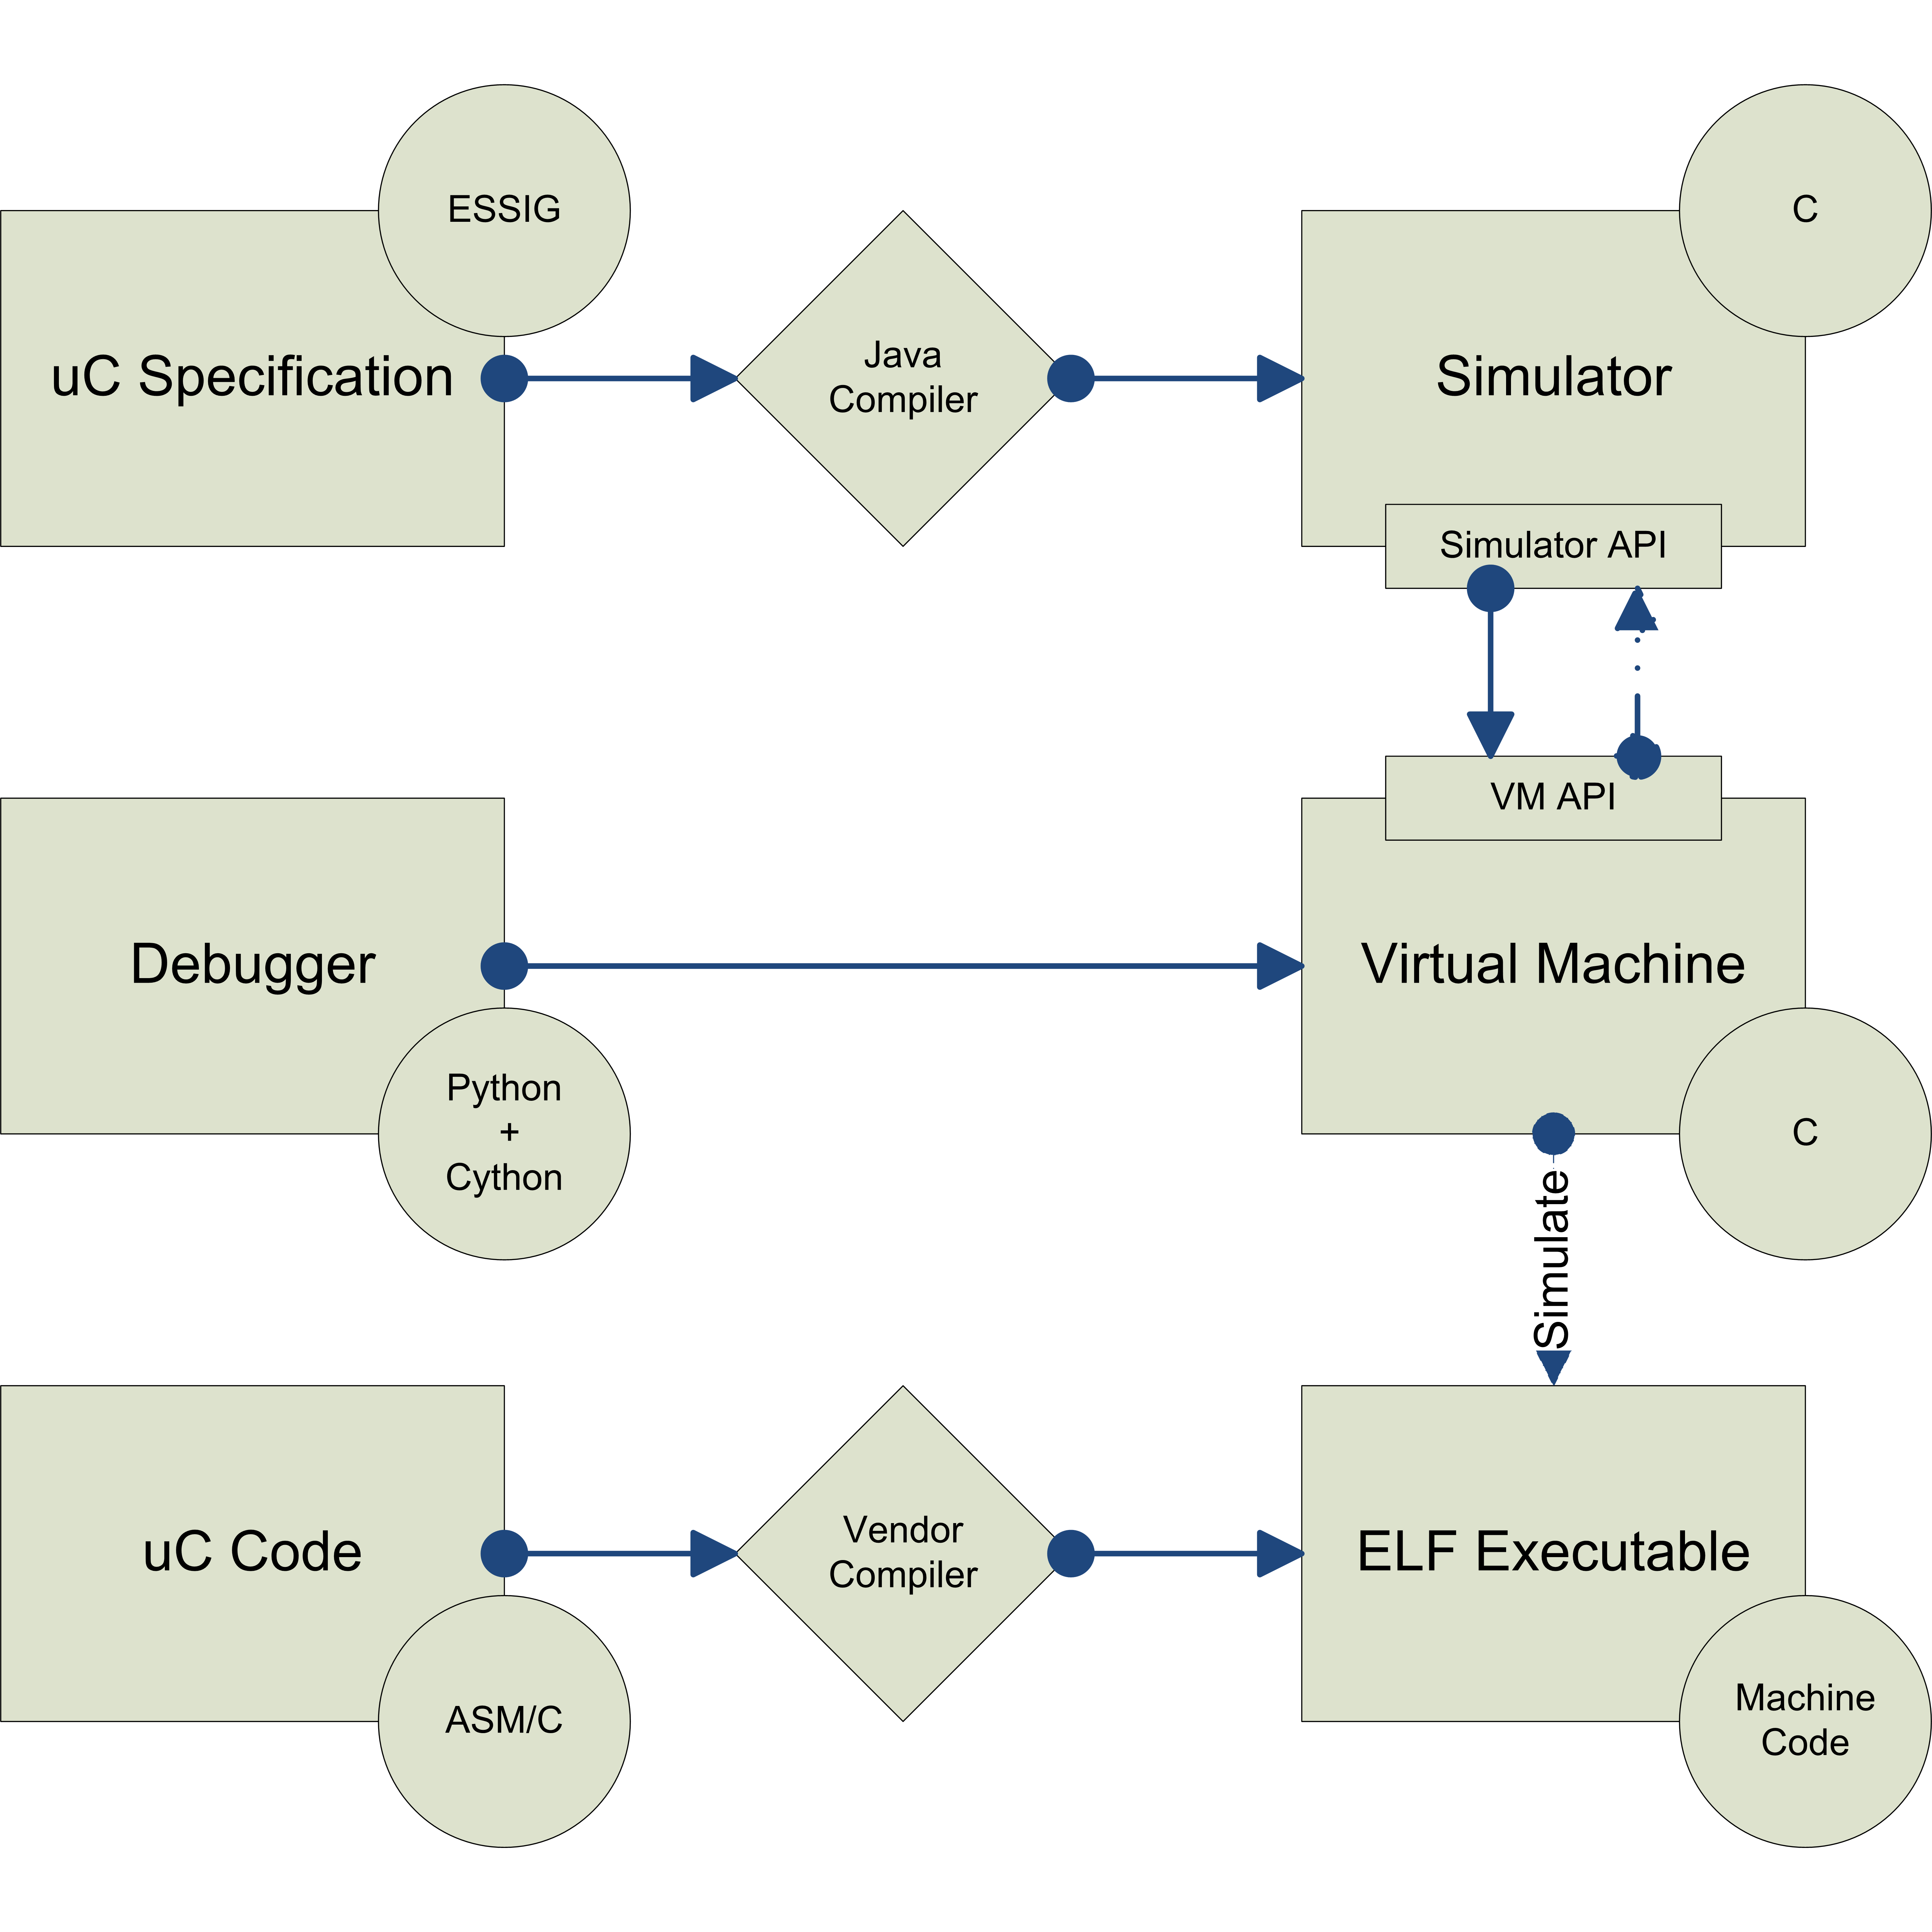
\includegraphics[width=500pt]{figures/tombstones.png}
\end{center}
\end{column}
\begin{column}{0.01\linewidth}\end{column}
\end{columns}
\end{block}
